\subsubsection{Manual}

Why do we adopt a manual way to split the entire program?

\begin{itemize}
    \item We avoid exceeding the stack depth limitation by only placing necessary data for the current chunk on the stack;
    \item We commit only the data used in the current chunk;
    \item We just need to implement gadgets to support ZKP verification as any computaion could generate a ZK proof;
    \item We use a Rust program to generate the input and output for each chunk;
    \item This approach minimizes costs when verifying the expected input and output on-chain;
    \item The logic of each chunk is readable.
\end{itemize}

\begin{figure}[ht] 
    \centering  
    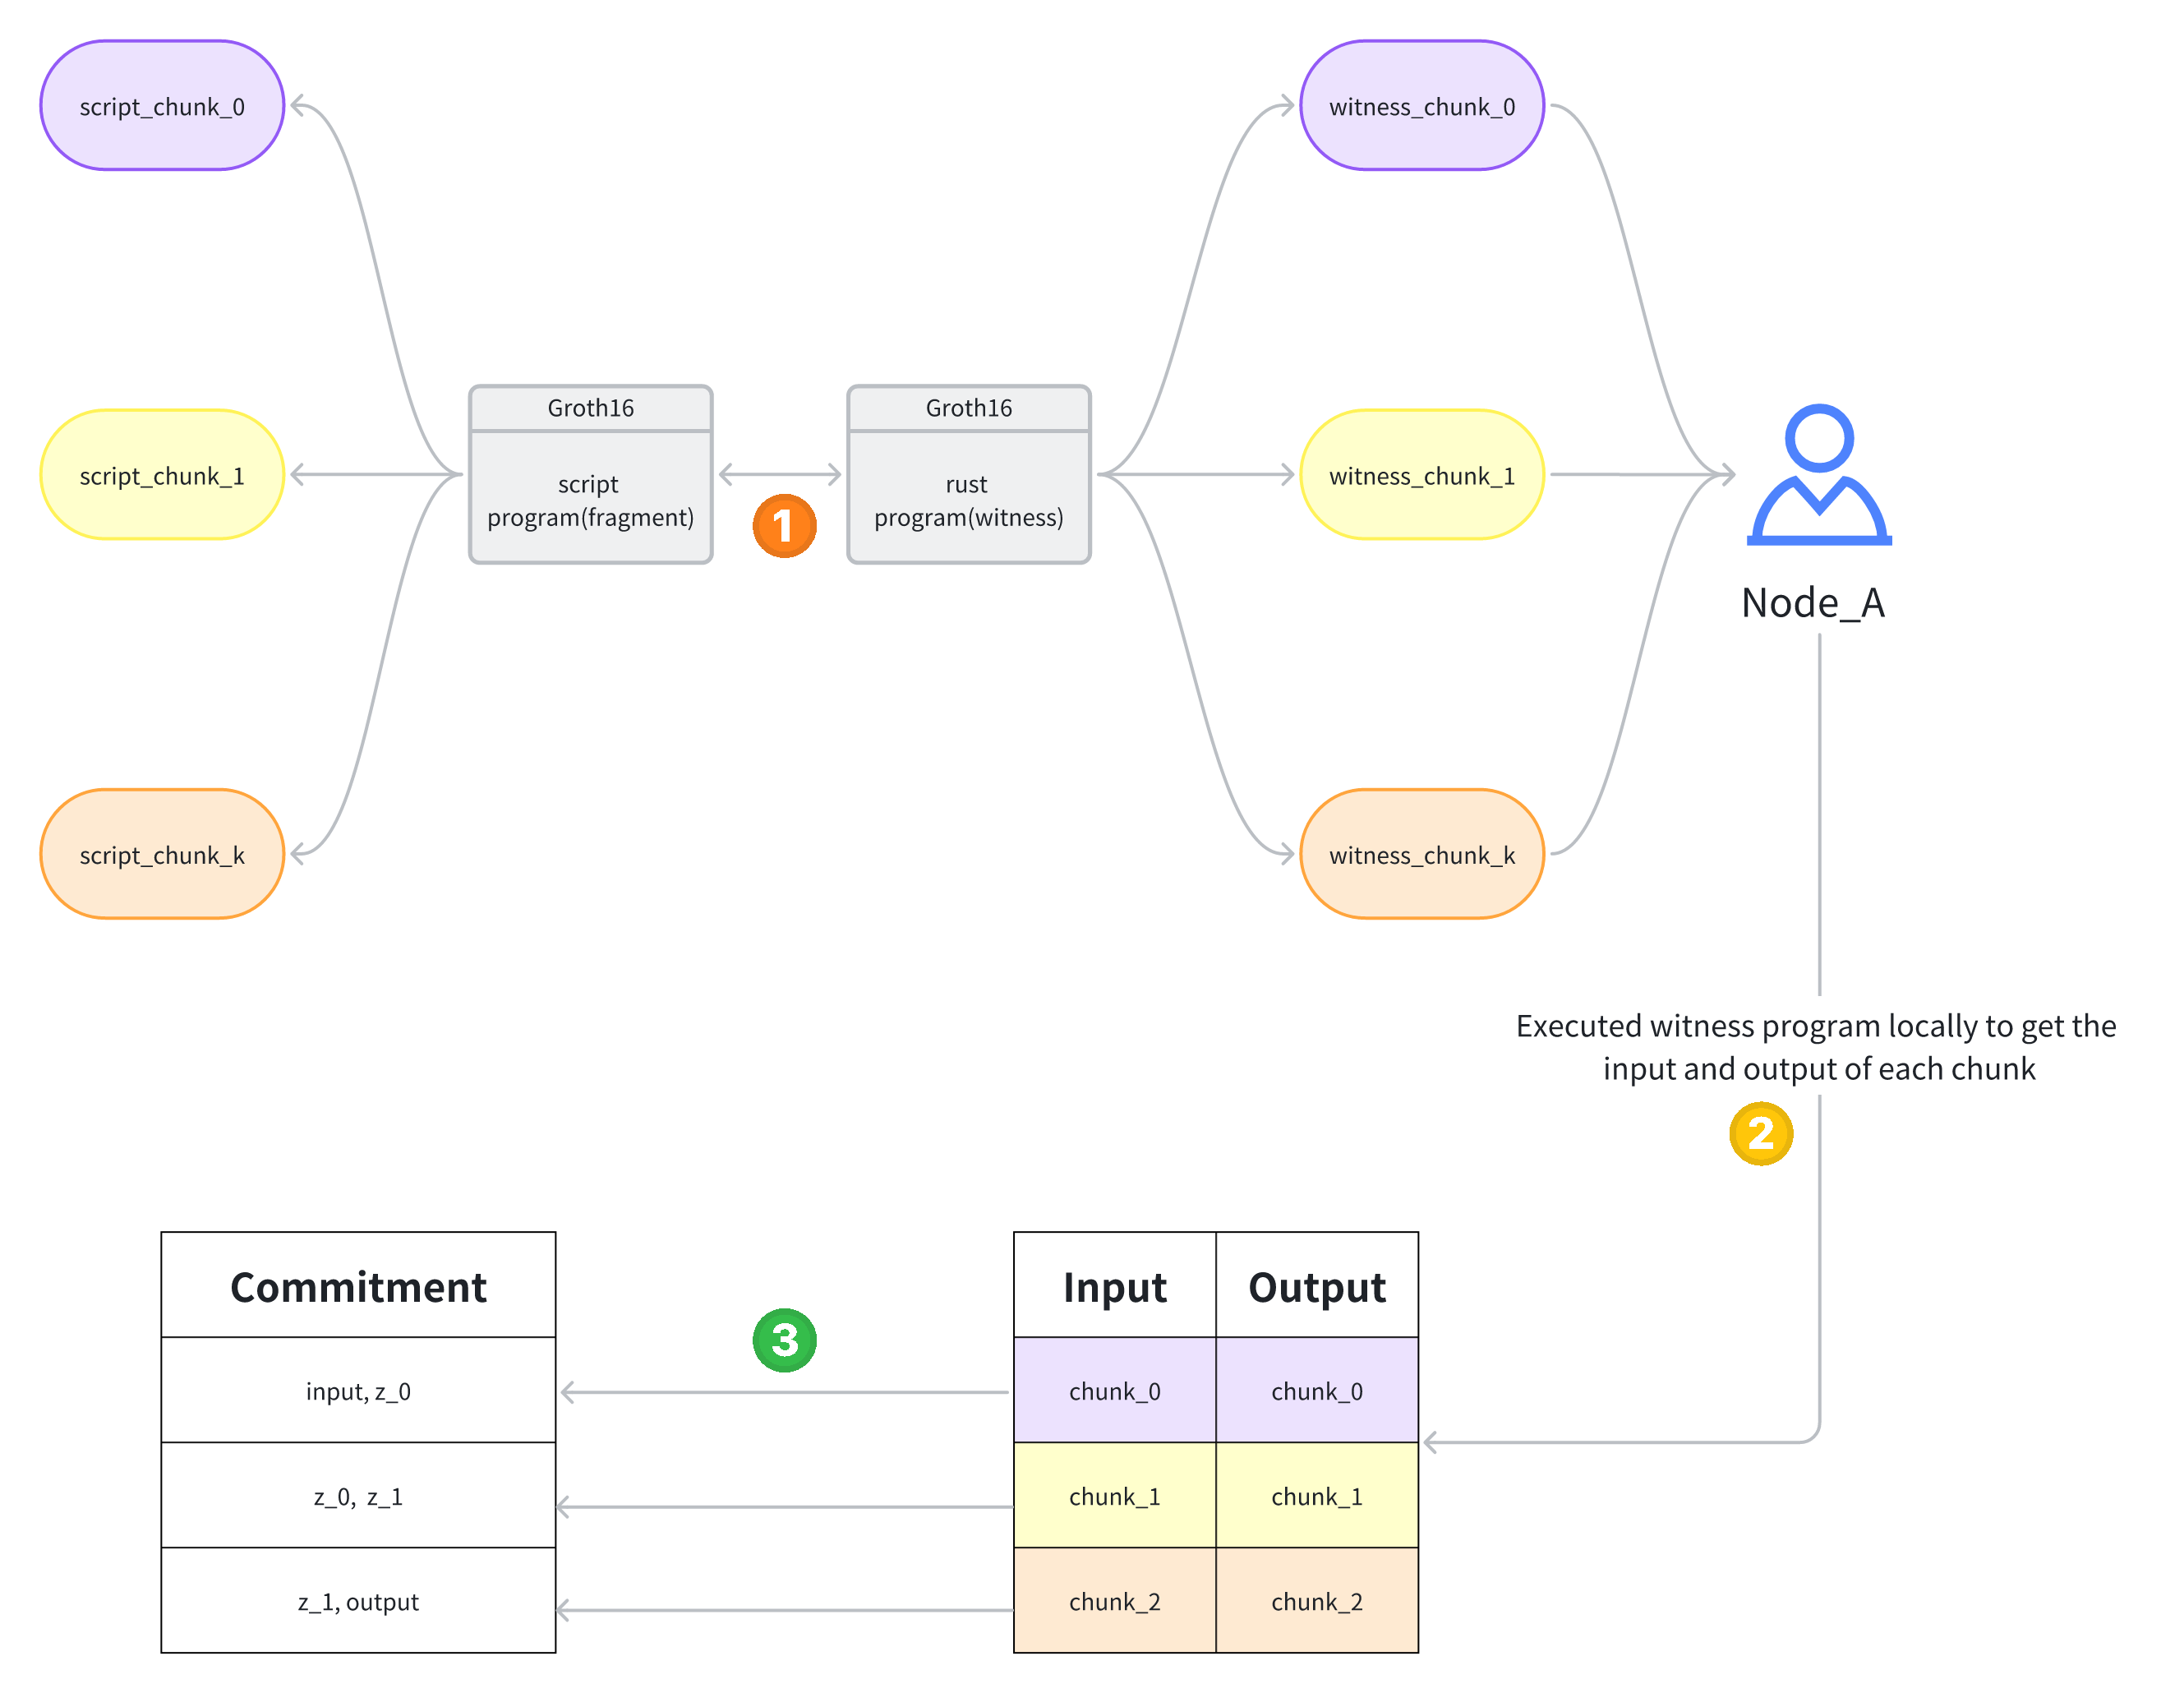
\includegraphics[width=0.65\columnwidth]{images/manually-fragment.png} 
    \caption{manual fragmentation}
    \label{fig:manually-fragment}
\end{figure}

While this approach may generate more chunks, as mentioned earlier, only one script chunk is executed on Bitcoin, so this is acceptable. The overall flow proceeds as follows:
\begin{itemize}
    \item We first concurrently implement the Rust and script versions of the Groth16 ZKP verification;
    \item The rust version includes the witness generation of each chunk;
    \item The script version includes all split chunks;
    \item We ensure each chunk meets the size and depth constraints;
    \item Node A executes the Rust program locally to generate inputs and outputs for each chunk;
    \item Node A commits all the inputs and outputs.
\end{itemize}
